\documentclass{scrartcl}
\usepackage{amssymb}
\usepackage{amsmath}
\usepackage{cancel}		%for strikethroughs
\usepackage{xparse}		%for modified strikethroughs
\usepackage{bm}			%for bolded quantifiers
\usepackage{tikz}
\usetikzlibrary{calc,intersections,through,backgrounds,patterns}
\usetikzlibrary{decorations.markings}
\usepackage{textcomp}

%via: tex.stackexchange.com/questions/20643/diagonal-strikeout-starting-too-low-and-ending-too-high
%if I specify the arguments in the text itself, it includes the arguments along with "La"
\DeclareDocumentCommand{\hcancel}{mO{-1pt}O{1pt}O{1pt}O{-3pt}}{%		%top "La"
	\tikz[baseline=(tocancel.base)]{
		\node[inner sep=0pt,outer sep=0pt] (tocancel) {#1};
		\draw ($(tocancel.south west)+(#2,#3)$) -- ($(tocancel.north east)+(#4,#5)$);
	}%
}%

\DeclareDocumentCommand{\lcancel}{mO{-1pt}O{1pt}O{2pt}O{-4pt}}{%		%bottom "La"
	\tikz[baseline=(tocancel.base)]{
		\node[inner sep=0pt,outer sep=0pt] (tocancel) {#1};
		\draw ($(tocancel.south west)+(#2,#3)$) -- ($(tocancel.north east)+(#4,#5)$);
	}%
}%

%To Do: add different translations; make a color version
%try out \reflectbox{E} for existential quantifier

\begin{document}

%\begin{figure}
%	\centering
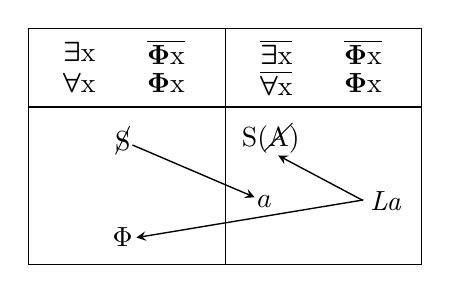
\begin{tikzpicture}

\draw (5,0) -- (0,0) -- (0,3) -- (5,3) -- (5,0);
\draw (0,2) -- (5,2);
\draw (2.5,3) -- (2.5,0);

%left side
\node at (0.65,2.7) {$\bm{\exists}\mathrm{x}$};
\node at (0.65,2.3) {$\bm{\forall}\mathrm{x}$};
\node at (1.75,2.7) {$\overline{\mathbf{\Phi}\mathrm{x}}$};
\node at (1.75,2.3) {$\mathbf{\Phi}\mathrm{x}$};

%right side
\node at (3.15,2.7) {$\overline{\bm{\exists}\mathrm{x}}$};
\node at (3.15,2.3) {$\overline{\bm{\forall}\mathrm{x}}$};
\node at (4.25,2.7) {$\overline{\mathbf{\Phi}\mathrm{x}}$};
\node at (4.25,2.3) {$\mathbf{\Phi}\mathrm{x}$};

%bottom symbols
\node (S) at (1.2,1.6)  {\cancel{S}};
\node (F) at (1.2,0.35) {$\Phi$};
\node (C) at (3.08,1.6) {S(\cancel{A})};
\node (A) at (3,0.8) 	{$a$};
\node (L) at (4.55,0.8) {\hcancel{\textit{La}}};

%\node (s') at (1.35,1.45) {.};	%dot next to S
  \node (s) at (1.2,1.57) {};	%dot next to S
%\node (f') at (1.45,0.35) {};	%dot next to \Phi
  \node (f) at (1.25,0.32) {};	%dot next to \Phi
%\node (c') at (3.08,1.3)  {.};	%dot under S(A)
  \node (c) at (3.05,1.45)  {};	%dot under S(A)
%\node (l'') at (4.18,0.8)  {.};	%dot next to La		%this one is a bit off
%\node (l') at (4.429,0.734) {.};	%dot next to La
\node (l') at (4.374,0.747) {};	%dot next to La			%arrow from C to L
  \node (l) at (4.38,0.84) {};	%dot next to La			%arrow from F to L
%\node (a') at (2.8,0.78)  {.};	%dot next to $a$
  \node (a) at (3,0.8)    {};	%dot next to $a$

\draw [->,>=stealth, line width=0.5pt] (l') edge (c) (l) edge (f) (s) edge (a);

\end{tikzpicture}
%	\caption{Lacan's sexuation formulas}
%\end{figure}

\vspace{1cm}

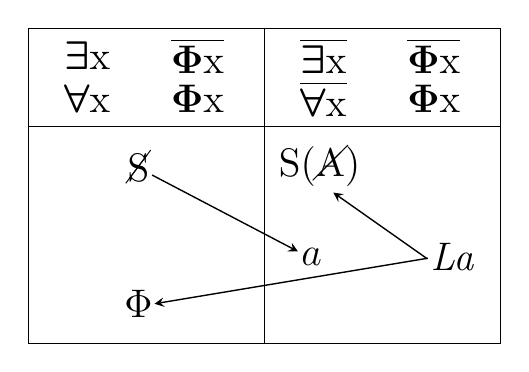
\begin{tikzpicture}

\draw (6,0) -- (0,0) -- (0,4) -- (6,4) -- (6,0);
\draw (0,2.75) -- (6,2.75);	%horizontal line
\draw (3,4) -- (3,0);		%vertical line

%left side
\node at (0.75,3.65) {{\Large $\bm{\exists}\mathrm{x}$}};
\node at (0.75,3.1) {{\Large $\bm{\forall}\mathrm{x}$}};
\node at (2.15,3.65) {{\Large $\overline{\mathbf{\Phi}\mathrm{x}}$}};
\node at (2.15,3.1) {{\Large $\mathbf{\Phi}\mathrm{x}$}};

%right side
\node at (3.75,3.65) {{\Large $\overline{\bm{\exists}\mathrm{x}}$}};
\node at (3.75,3.1) {{\Large $\overline{\bm{\forall}\mathrm{x}}$}};
\node at (5.15,3.65) {{\Large $\overline{\mathbf{\Phi}\mathrm{x}}$}};
\node at (5.15,3.1) {{\Large $\mathbf{\Phi}\mathrm{x}$}};

%bottom symbols
\node (S) at (1.4,2.25)  {{\Large \cancel{S}}};
\node (F) at (1.4,0.5)  {{\Large $\Phi$}};
\node (C) at (3.7,2.25) {{\Large S(\cancel{A})}};
\node (A) at (3.6,1.1) {{\Large $a$}};
\node (L) at (5.4,1.1)  {{\Large \lcancel{\textit{La}}}};

\node (s) at (1.45,2.2) {};	%dot next to S
\node (f) at (1.48,0.48)  {};	%dot next to \Phi
\node (c) at (3.75,2) {};	%dot under S(A)
\node (a) at (3.55,1.1)  {};	%dot next to $a$
\node (l) at (5.2,1.1)  {};	%dot next to La			%arrow from F to L
\node (l') at (5.194,0.983)  {};	%dot next to La			%arrow from S(A) to L

\draw [->,>=stealth, line width=0.5pt] (l') edge (c) (l) edge (f) (s) edge (a);

\end{tikzpicture}

\end{document}